\documentclass{article}

\usepackage{pgfplots}

\usepgfplotslibrary{fillbetween}


\begin{document}

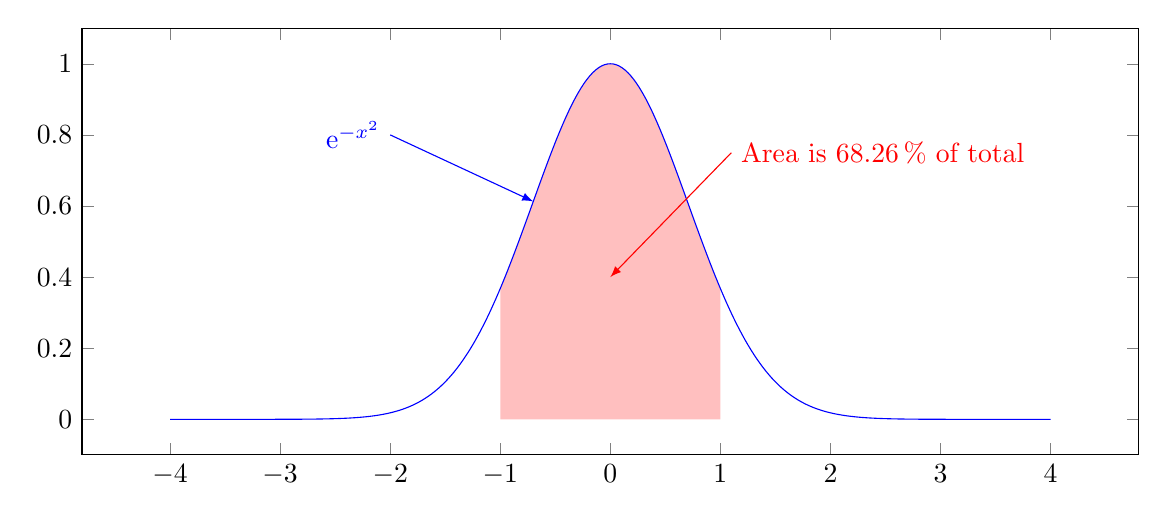
\begin{tikzpicture}[
  declare function = { bell(\x) = exp(-\x^2); }
  ]

\begin{axis}[
    width=15cm,
    height=7cm]

%% Plot bell curve
\addplot [blue, mark=none, samples=301, name path=f,domain=-4:4] { bell(\x) };

%% Just a path over the x axis
\path[name path=xaxis] (axis cs:-4,0) -- (axis cs:4,0);

%% Fill the area between x axis and bell curve, from x = -1 to x = 1 (1 sigma)
\addplot [thick, fill=red, fill opacity=0.25]
              fill between[of=f and xaxis, soft clip={domain=-1:1}];
        
%% Show the 1 sigma area
\draw[latex-,red] (axis cs:0.0,0.4) -- (axis cs:1.1,0.75) node[right] {Area is 68.26\,\% of total};

% Show function
\draw[latex-,blue] (axis cs:-0.7,{bell(-0.7)}) -- (axis cs:-2,0.8) node[left] {$\mathrm{e}^{-x^2}$};

\end{axis}

\end{tikzpicture}

\end{document}